% --------------------------------------------------------------------------------

\begin{exercise}

Für ein beschränktes Lipschitz-Gebiet $\Omega \subset \R^2$ definieren wir den Hilbertraum

\begin{align*}
  H(\curl, \Omega)
  :=
  \Bbraces{\xi \in [L^2(\Omega)]^2 | \curl \xi \in L^2(\Omega)}, 
  \quad
  (\xi, \zeta)_{H(\curl)}
  :=
  (\xi, \zeta)_{L^2(\Omega)} + (\curl \xi, \curl \zeta)_{L^2(\Omega)}, 
\end{align*}

mit $\curl \xi := \frac{\partial \xi_2}{\partial x} - \frac{\partial \xi_1}{\partial y}$ für $\xi(x, y) = (\xi_1(x, y), \xi_2(x, y))^\top$.
Weiter sei $X := H^1_0(\Omega) \times H(\curl, \Omega)$ ein Hilbert-Raum wie in Aufgabe 6.

Für ein $c \geq 0$ und $f \in L^2(\Omega)$ sei das folgende Variationsproblem gegeben: Finden Sie $(u, \xi) \in X$ sodass für alle $(v, \zeta) \in X$

\begin{align}
  \Int[\Omega]{(\nabla u - \xi) \cdot (\nabla v - \zeta)}{x}
  +
  c \Int[\Omega]{\xi \cdot \zeta}{x}
  +
  \Int[\Omega]{\curl \xi \curl \zeta}{x}
  =
  \Int[\Omega]{f v}{x}
\end{align}

\begin{enumerate}[label = \textbf{\alph*)}]

  \item Zeigen Sie mit Hilfe des Lemmas von Lax-Milgram, dass für $c > 0$ das Problem eine eindeutige Lösung hat.
  Verwenden Sie dazu am besten die Young Ungleichung $-ab \geq - \frac{\varepsilon}{2} a^2 - \frac{1}{2\varepsilon}b^2$ für geeignete $a, b \in \R$ und $\varepsilon > 0$.

  \item Es sei nun $c = 0$.
  Zeigen Sie durch geschicktes Wählen von $(u, \xi) \in X$, dass das Problem nicht koerziv ist.
  \textit{Hinweis}:
  Was gilt für $\curl \nabla u$?

  \item Begründen Sie mit den Funktionen $\xi_\varepsilon \in [H^1(\Omega)]^2$ definiert durch $\xi_\varepsilon(x, y) := (\sin(\frac{1}{\varepsilon}x), 0)^\top$ mit $\varepsilon > 0$, dass das Problem auf dem Produktraum $\hat{X} := H^1_0(\Omega) \times [H^1(\Omega)]^2$ mit $c > 0$ nicht koerziv und damit nicht wohlgestellt ist.

\end{enumerate}

\end{exercise}

% --------------------------------------------------------------------------------

\begin{solution}

\phantom{}

\begin{align*}
  \pbraces
  {
    \begin{pmatrix}
      u \\ \xi
    \end{pmatrix},
    \begin{pmatrix}
      v \\ \zeta
    \end{pmatrix}
  }_X
  & =
  (u, v)_{H^1(\Omega)}
  +
  (\xi, \zeta)_{H(\curl, \Omega)} \\
  & =
  (u, v)_{L^2(\Omega)}
  +
  (\nabla u, \nabla v)_{L^2(\Omega)}
  +
  (\xi, \zeta)_{L^2(\Omega)}
  +
  (\curl \xi, \curl \zeta)_{L^2(\Omega)}
\end{align*}

\begin{align*}
  \implies
  \norm[X]
  {
    \begin{pmatrix}
      u \\ \xi
    \end{pmatrix}
  }
  & =
  \pbraces
  {
    \begin{pmatrix}
      u \\ \xi
    \end{pmatrix},
    \begin{pmatrix}
      u \\ \xi
    \end{pmatrix}
  }_X^{1/2} \\
  & =
  \pbraces
  {
    (u, u)_{L^2(\Omega)}
    +
    (\nabla u, \nabla u)_{L^2(\Omega)}
    +
    (\xi, \xi)_{L^2(\Omega)}
    +
    (\curl \xi, \curl \xi)_{L^2(\Omega)}
  }^{1/2} \\
  & =
  \pbraces
  {
    \norm[L^2(\Omega)]{u}^2
    +
    \norm[L^2(\Omega)]{\nabla u}^2
    +
    \norm[L^2(\Omega)]{\xi}^2
    +
    \norm[L^2(\Omega)]{\curl \xi}^2
  }^{1/2}
\end{align*}

\begin{enumerate}[label = \textbf{\alph*)}]

  \item \phantom{}

  \begin{center}
    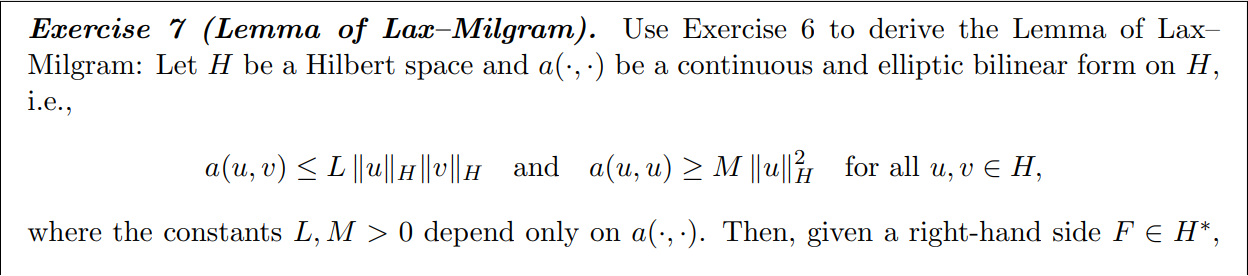
\includegraphics[width = 0.75 \textwidth]{NumPDEs/NumPDEs - Exercise 7.1 (Lemma of Lax-Milgram).png} \\
    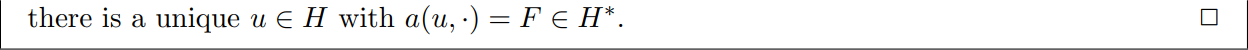
\includegraphics[width = 0.75 \textwidth]{NumPDEs/NumPDEs - Exercise 7.2 (Lemma of Lax-Milgram).png}
  \end{center}

  \begin{align*}
    a
    \pbraces
    {
      \begin{pmatrix}
        u \\ \xi
      \end{pmatrix},
      \begin{pmatrix}
        v \\ \zeta
      \end{pmatrix}
    }
    & :=
    \Int[\Omega]{(\nabla u - \xi) \cdot (\nabla v - \zeta)}{x}
    +
    c \Int[\Omega]{\xi \cdot \zeta}{x}
    +
    \Int[\Omega]{\curl \xi \curl \zeta}{x} \\
    F
    \begin{pmatrix}
      v \\ \xi
    \end{pmatrix}
    & :=
    \Int[\Omega]{f v}{x}
  \end{align*}

  \begin{enumerate}[label = \arabic*.]

    \item Stetigkeit von $a$:
    
    Auf dem $\R^3$ sind die Normen $\norm[1]{\cdot}$ und $\norm[2]{\cdot}$ äquivalent.
    Wir erhalten also eine Konstante $C > 0$, sodass $\norm[1]{\cdot} \leq C \norm[2]{\cdot}$.

    \begin{align*}
      \norm[1]{\cdot}
      \sim
      \norm[2]{\cdot}
      ~\text{auf $\R^3$}~
      \implies
      \Exists C > 0:
      \norm[1]{\cdot}
      \leq
      C
      \norm[2]{\cdot}
    \end{align*}

    \begin{align*}
      a
      \pbraces
      {
        \begin{pmatrix}
          u \\ \xi
        \end{pmatrix},
        \begin{pmatrix}
          v \\ \zeta
        \end{pmatrix}
      }
      & =
      \Int[\Omega]{(\nabla u - \xi) \cdot (\nabla v - \zeta)}{x}
      +
      c \Int[\Omega]{\xi \cdot \zeta}{x}
      +
      \Int[\Omega]{\curl \xi \curl \zeta}{x} \\
      & \stackrel
      {
        \mathrm{CSB}
      }{\leq}
      \norm[L^2(\Omega)]{\nabla u - \xi}
      \norm[L^2(\Omega)]{\nabla v - \zeta} \\
      & \quad
      +
      c
      \norm[L^2(\Omega)]{\xi}
      \norm[L^2(\Omega)]{\zeta}
      +
      \norm[L^2(\Omega)]{\curl \xi}
      \norm[L^2(\Omega)]{\curl \zeta} \\
      & \leq
      \pbraces
      {
        \norm[L^2(\Omega)]{\nabla u}
        +
        \norm[L^2(\Omega)]{\xi}
      }
      \pbraces
      {
        \norm[L^2(\Omega)]{\nabla u}
        +
        \norm[L^2(\Omega)]{\zeta}
      } \\
      & \quad
      +
      c
      \norm[L^2(\Omega)]{\xi}
      \norm[L^2(\Omega)]{\zeta}
      +
      \norm[L^2(\Omega)]{\curl \xi}
      \norm[L^2(\Omega)]{\curl \zeta} \\
      & \leq
      2 \max \Bbraces{1, c} \\
      & \quad
      \pbraces
      {
        \norm[H^1(\Omega)]{u}
        +
        \norm[L^2(\Omega)]{\xi}
        +
        \norm[L^2(\Omega)]{\curl \xi}
      } \\
      & \quad
      \pbraces
      {
        \norm[H^1(\Omega)]{v}
        +
        \norm[L^2(\Omega)]{\zeta}
        +
        \norm[L^2(\Omega)]{\curl \zeta}
      } \\
      & =
      2 \max \Bbraces{1, c} \\
      & \quad
      \norm[1]
      {
        \pbraces
        {
          \norm[H^1(\Omega)]{u},
          \norm[L^2(\Omega)]{\xi},
          \norm[L^2(\Omega)]{\curl \xi}
        }^\top
      } \\
      & \quad
      \norm[1]
      {
        \pbraces
        {
          \norm[H^1(\Omega)]{v},
          \norm[L^2(\Omega)]{\zeta},
          \norm[L^2(\Omega)]{\curl \zeta}
        }^\top
      } \\
      & \leq
      2 \max \Bbraces{1, c} C^2 \\
      & \quad
      \norm[2]
      {
        \pbraces
        {
          \norm[H^1(\Omega)]{u},
          \norm[L^2(\Omega)]{\xi},
          \norm[L^2(\Omega)]{\curl \xi}
        }^\top
      } \\
      & \quad
      \norm[2]
      {
        \pbraces
        {
          \norm[H^1(\Omega)]{v},
          \norm[L^2(\Omega)]{\zeta},
          \norm[L^2(\Omega)]{\curl \zeta}
        }^\top
      } \\
      & =
      2 \max \Bbraces{1, c} C^2 \\
      & \quad
      \pbraces
      {
        \norm[H^1(\Omega)]{u}^2
        +
        \norm[L^2(\Omega)]{\xi}^2
        +
        \norm[L^2(\Omega)]{\curl \xi}^2
      }^{1/2} \\
      & \quad
      \pbraces
      {
        \norm[H^1(\Omega)]{v}^2
        +
        \norm[L^2(\Omega)]{\zeta}^2
        +
        \norm[L^2(\Omega)]{\curl \zeta}^2
      }^{1/2} \\
      & =
      2 \max \Bbraces{1, c} C^2
      \norm[X]
      {
        \begin{pmatrix}
          u \\ \xi
        \end{pmatrix}
      }
      \norm[X]
      {
        \begin{pmatrix}
          v \\ \zeta
        \end{pmatrix}
      }
    \end{align*}

    \item Elliptizität von $a$:
    
    \includegraphicsunboxed{PDEs/PDEs_-_Satz_5-11_(Poincare-Ungleichung).png}

    Die Poincaré-Ungleichung von \cite{PDEs} liefert uns ein $C_p > 0:$

    \begin{align*}
      \norm[H^1(\Omega)]{u}^2
      =
      \norm[L^2(\Omega)]{u}^2
      +
      \norm[L^2(\Omega)]{\nabla u}^2
      \leq
      (C_p + 1)^2 \norm[L^2(\Omega)]{\nabla u}^2
      \implies
      \norm[L^2(\Omega)]{\nabla u}
      \geq
      \frac{1}{C_p + 1}
      \norm[H^1(\Omega)]{u}^2.
    \end{align*}

    In der folgenden Abschätzung verwenden wir die Young Ungleichung mit $\varepsilon \in \pbraces{\frac{1}{c + 1}, 1}$.
    
    \begin{align*}
      a
      \pbraces
      {
        \begin{pmatrix}
          u \\ \xi
        \end{pmatrix},
        \begin{pmatrix}
          u \\ \xi
        \end{pmatrix}
      }
      & =
      \Int[\Omega]{(\nabla u - \xi) \cdot (\nabla u - \xi)}{x}
      +
      c \Int[\Omega]{\xi \cdot \xi}{x}
      +
      \Int[\Omega]{\curl \xi \curl \xi}{x} \\
      & =
      \norm[L^2(\Omega)]{\nabla u - \xi}^2
      +
      c \norm[L^2(\Omega)]{\xi}^2
      +
      \norm[L^2(\Omega)]{\curl \xi}^2 \\
      & \geq
      \pbraces
      {
        \norm[L^2(\Omega)]{\nabla u}
        -
        \norm[L^2(\Omega)]{\xi}
      }^2
      +
      c \norm[L^2(\Omega)]{\xi}^2
      +
      \norm[L^2(\Omega)]{\curl \xi}^2 \\
      & =
      \norm[L^2(\Omega)]{\nabla u}^2
      -
      2
      \norm[L^2(\Omega)]{\nabla u}
      \norm[L^2(\Omega)]{\xi}
      +
      \norm[L^2(\Omega)]{\xi}^2
      +
      c
      \norm[L^2(\Omega)]{\xi}^2
      +
      \norm[L^2(\Omega)]{\curl \xi}^2 \\
      & \stackrel
      {
        \mathrm{Y}
      }{\geq}
      \norm[L^2(\Omega)]{\nabla u}^2
      -
      \varepsilon
      \norm[L^2(\Omega)]{\nabla u}^2
      -
      \frac{1}{\varepsilon}
      \norm[L^2(\Omega)]{\xi}^2
      +
      \norm[L^2(\Omega)]{\xi}^2
      +
      c
      \norm[L^2(\Omega)]{\xi}^2
      +
      \norm[L^2(\Omega)]{\curl \xi}^2 \\
      & =
      (1 - \varepsilon)
      \norm[L^2(\Omega)]{\nabla u}^2
      +
      \pbraces{1 + c - \frac{1}{\varepsilon}}
      \norm[L^2(\Omega)]{\xi}^2
      +
      \norm[L^2(\Omega)]{\curl \xi}^2 \\
      & \geq
      \frac{1 - \varepsilon}{(C_p + 1)^2}
      \norm[H^1(\Omega)]{\nabla u}^2
      +
      \pbraces{1 + c - \frac{1}{\varepsilon}}
      \norm[L^2(\Omega)]{\xi}^2
      +
      \norm[L^2(\Omega)]{\curl \xi}^2 \\
      & \geq
      \min
      \Bbraces
      {
        \frac{1 - \varepsilon}{(C_p + 1)^2},
        1 + c - \frac{1}{\varepsilon},
        1
      }
      \pbraces
      {
        \norm[H^1(\Omega)]{\nabla u}^2
        +
        \norm[L^2(\Omega)]{\xi}^2
        +
        \norm[L^2(\Omega)]{\curl \xi}^2
      } \\
      & =
      \min
      \Bbraces
      {
        \frac{1 - \varepsilon}{(C_p + 1)^2},
        1 + c - \frac{1}{\varepsilon},
        1
      }
      \norm[X]
      {
        \begin{pmatrix}
          u \\ \xi
        \end{pmatrix}
      }^2
    \end{align*}

    Wir sind fertig, weil $c > 0$.

    \item Stetigkeit von $F$:
    
    \begin{align*}
      F
    \begin{pmatrix}
      v \\ \xi
    \end{pmatrix}
    =
    \Int[\Omega]{f v}{x}
    \stackrel
    {
      \mathrm{CSB}
    }{\leq}
    \norm[L^2(\Omega)]{f}
    \norm[L^2(\Omega)]{v}
    \leq
    \norm[L^2(\Omega)]{f}
    \norm[X]
    {
      \begin{pmatrix}
        v \\ \xi
      \end{pmatrix}  
    }
    \end{align*}

  \end{enumerate}

\end{enumerate}

\end{solution}

% --------------------------------------------------------------------------------
